The contribution of our proposed system will be demonstrated on a case study which corresponds to real problems the biochemists are currently facing. 
Later, we present the detailed performance analysis.

\subsection{Case Study~--~Real-time visual exploration of MD simulation}
The case study deals with the situation when the biochemists want to visually explore the inner processes occurring inside the molecule. 
An example of such a process can be the penetration of a small molecule (ligand) into the active site of the protein where the ligand reacts with the protein and the product of such reaction can form the basis of new chemical matters, e.g., new drugs. 
The current workflow generating the desired visual appearance of the animation showing such processes consists of many trial and error attempts, which makes the whole workflow very lengthy. 
To describe this process in more detail, the biochemists start in the first time step of the whole simulation and try to manually determine the best viewpoint.
As the view inside the molecule, where the processes usually occur, is crucial, they utilize clip planes to achieve this.
The manual setting of the clip planes introduces other possible error to the final animation.
The dynamic movements of the molecule can cause its rotation and the clip plane settings in the first time step might have completely wrong positions in the following steps .
When all the visual parameters are set in the first frame (Fig.~\ref{fig:animation}), the biochemists use an offline rendering tool for generating the whole animation.
In this phase they do not posses any control of this process so it is impossible to detect an error inside the animation and stop the generation.
These errors, such as occlusions or wrong clip plane positions, are detected when playing the final animation.
The only solution is to adjust the input settings and launch the whole process once again.
For better illustration, in case of the example video (from which Figure~\ref{fig:animation} (top) is captured), it took two days to produce the solution which comprehensibly shows the whole process of ligand penetration to the protein active site.

Our new system is able to overcome the following limitations of the above-described workflow:
\begin{itemize} 
\item The MD simulation can be observed in real time which enables the user to interactively adjust the appearance and viewpoint.
\item The highly transparent molecular surface removes the necessity of using clip planes.
\item The user has the full control of the animation process so we completely remove the trial and error phase of the workflow. 
\end{itemize}

In consequence, our system enables to reach similar results in real-time. 
In one aspect it even overcomes the existing solution as the users can interactively manipulate with the scene on the fly~--~perform scene transformations, change the appearance of the protein and ligand, or change the probe size used for the generation of protein surface.

Figure \ref{fig:animation} (bottom) shows one time step of the animation generated using the same dataset as for the top part of this Figure.

\begin{figure}[htb]
  \centering
  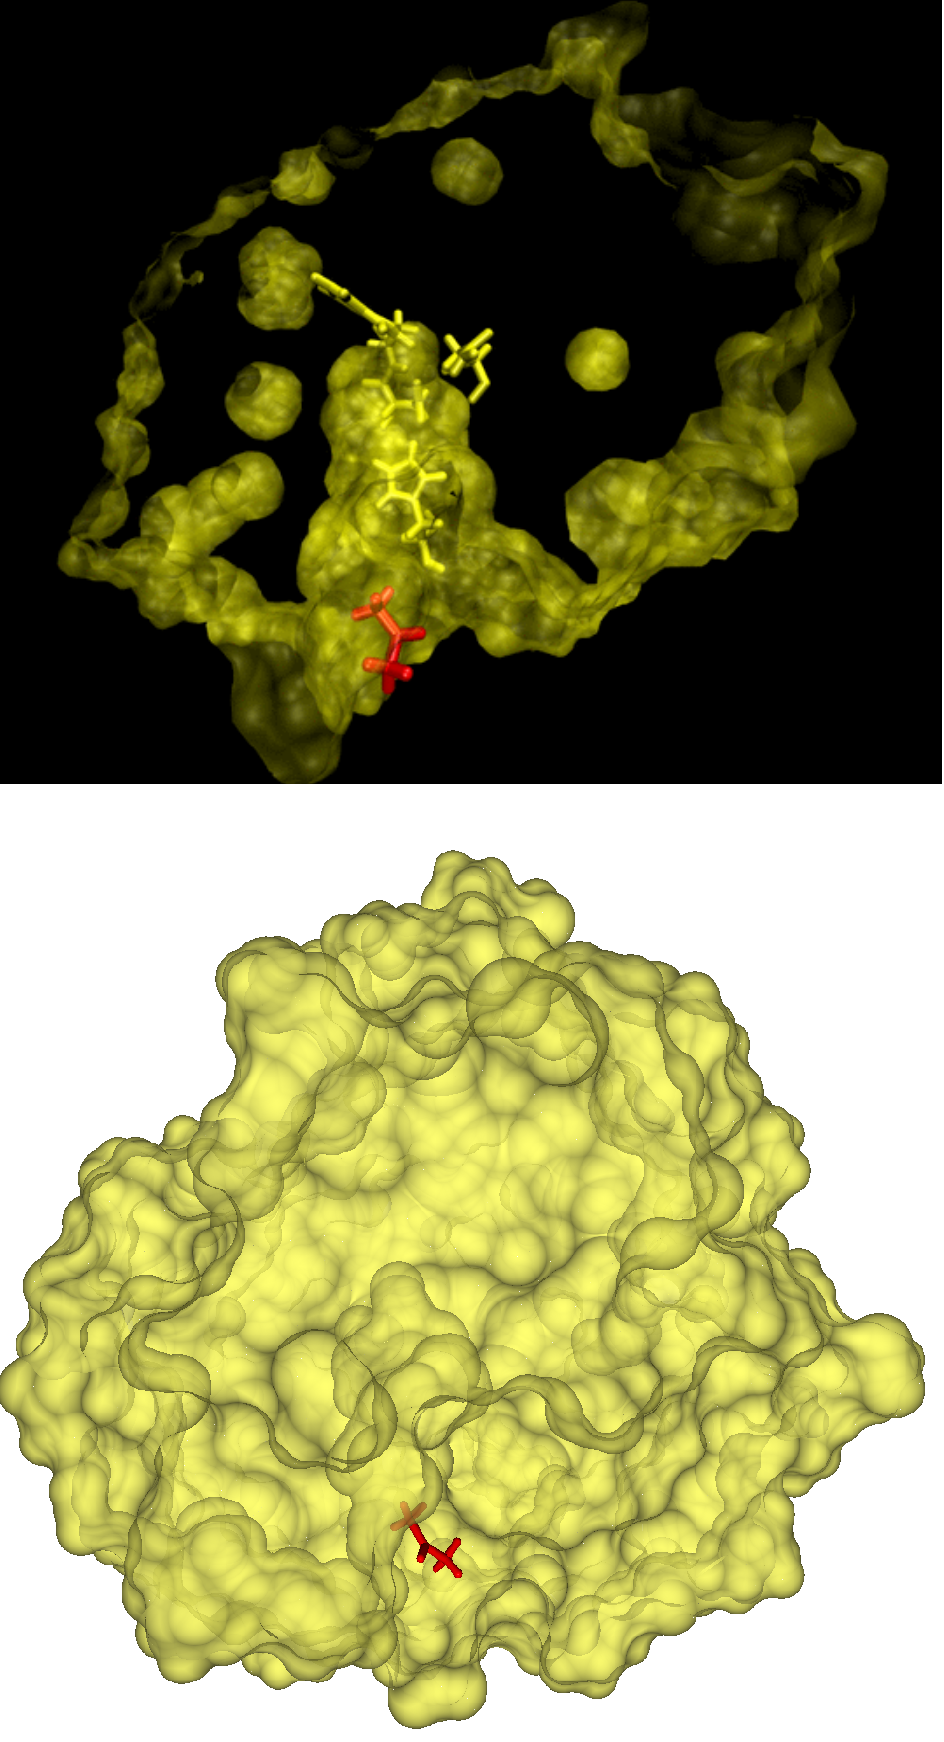
\includegraphics[width=2.5in]{image/animation.png}
  \caption{Top: One time step from the animation aiming to show the penetration of the ligand to the protein active site. For better insight, different representations of the molecule and the ligand, surface transparency, clip plane, and different coloring was used. Bottom: One time step of the animation generated using our algorithm. It shows the same molecule and its dynamics. By enabling the interactive manipulation with the scene within the animation, the user can clearly see the transportation route without the necessity to use any clip plane.}
	\label{fig:animation}
\end{figure}

When the results of the algorithm were evaluated by the domain experts, they confirmed that our solution is highly practical with respect to the described task because the time to complete this task is reduced dramatically.
Moreover, they also appreciated the visual appearance which they considered to be more appealing than the previous solutions.
They confirmed that our approach can be directly used for creating presentation materials, such as images to publications or animations for presentations.

The domain experts were also asked to identify the weak points of our current solution.
They agreed that when using a highly transparent molecular surface, the position of a ligand can be hard to assess when using only one viewpoint.
In other words, the user has to manipulate with the structure in order to decide if the ligand is still located in the outer solvent or if it already penetrated to the inner part of the protein.
However, this situation is caused due to the transparency itself and a solution has to be based on a combination with other methods.
This opens one of the possible directions for the future extension.

\subsection{Performance Analysis}
\label{sec:performance}

\begin{itemize}
  \item Performance analysis
  \item Pros \& cons
  \item Limits
\end{itemize}

We tested our technique on commodity hardware to show that it enables the users to solve their tasks in real-time without high hardware requirements.
\textcolor{red}{Test also on high-end hardware --- GTX 980?}
The tests were performed using Intel Core i5 760 (2.80 GHz) with 4 GB of RAM and NVIDIA GeForce 680 GTX with 4 GB of VRAM as a graphics card.
For rendering, we used resolution of 1024 $\times$ 768 and we tried to fit the molecule such that it covered most of the image.
Regarding transparency, we limited the maximum depth complexity to 24 fragments per pixel.
The results of our measurements for static molecules are presented in Table~\ref{tab:static}.

\setlength{\tabcolsep}{4.4pt}

\begin{table}[htb]
  \caption{Performance of our technique for static structures.}
  \label{tab:static}
  \scriptsize
  \begin{center}
    \begin{tabular}{ccccccc}
      Molecule & \# Atoms & CB & SG & AO+Area & Ray-casting & Total \\
			%        &       & buildup  & graph   & Area & casting &       \\
							&       & (ms)     & (ms)    & (ms) & (ms) & (FPS) \\
    \hline
      1OGZ &  {\tweakedsim}1000 &  4.1 & 0.2 & 0.2 & 15.7 (36.7\%) & 31.0 \\
      1VIS &  {\tweakedsim}2500 &  6.1 & 0.8 & 0.2 & 39.3 (52.7\%) & 16.4 \\
      4ADJ & {\tweakedsim}10000 & 21.1 & 4.3 & 0.4 & 97.7 (41.5\%) &  6.9
    \end{tabular}
  \end{center}
\end{table}

Our technique was implemented mainly using OpenGL employing GLSL compute shaders as GPU kernels.
We also utilize OpenCL to accelerate a kernel which computes positions of spherical triangles in the original algorithm \cite{krone2011parallel}.
The GLSL implementation of this kernel performed for a molecule with {\tweakedsim}10000 atoms is about 5x slower than the OpenCL/CUDA one.
From the tests we did, we assume that the key of such performance loss is the extensive use of the global memory in the kernel which is handled differently in OpenGL and OpenCL/CUDA.

From the results, it can be seen that in terms of performance, the main limitation of our technique is ray-casting of the computed surface.
More specifically, the demanding parts are rendering of spherical and toroidal patches that take together 75-80\% of the whole rendering time.
We anticipate that the performance of ray-casting these patches could be improved by using tighter bounding boxes for them when splatting.
In fact, we employ bounding squares for both spheres containing spherical patches and visibility spheres containing visible parts of tori.
In this way, the computation of ray-primitive intersection is evaluated multiple times for spheres and tori that form more than one surface patch.